\chapter{Experiments and Results}
\label{cha:ResearchAndResults}

{\it In this chapter, the results from the experiments will be presented and discussed. Section \ref{sec:results} contains the actual results created by running each scenario. The setup of the experiment is explained in section \ref{sec:experimentalSetup}, it explains the setup and which parameters have been used to run the experiments.
Section \ref{sec:discussion} will discuss the results seen in section \ref{sec:results}, and a discussion on the differences between the results from the simulator and the physical robots.}

\section{Experimental Plan}
\label{sec:experimentalPlan}
To be able to test whether the robots are behaving like the Boids, and graphs are plotted to compare the difference between the Boids and the robots. 
Three scenarios or three different starting position will be used as explained in section \ref{sec:experimentalSetup}.
For the physical experiment with the robots, each scenario will be ran ten times to generate the graphs for the results, while only five runs will be used for the results.
%TODO, write about how the experiments were ran.

%from template: Trying and failing is a major part of research. However, to have a chance of success you need a plan driving the experimental research, just as you need a plan for your literature search. Further, plans are made to be revised and this revision ensures that any further decisions made are in line with the work already completed. The plan should include what experiments or series of experiments are planned and what question the individual or set of experiments aim to answer. Such questions should be connected to your research questions so that in the evaluation of your results you can discuss the results wrt to the research questions.  

\section{Experimental Setup}
\label{sec:experimentalSetup}
%In this section, the setup for the experiment will be explained, and which parameters have been used to run the experiments. 
This section explains the setup of each scenario, where each robot is placed in the sandbox, which way it is rotated and where the obstacle is placed. Each scenario have a purpose to demonstrate, which will be explained more in detail.
In this experiment, four robots and one obstacle is used inside a sandbox. Each robots needs to have an extra layer on top of them so the red and green post it note does not fall off as seen in figure \ref{fig:robot0}. The robots moves inside a sandbox, which is watched by a web camera from above.

For this project experiment, three scenarios have been used to create the results seen in section \ref{sec:results}.
\label{sec:scenario}
\begin{figure}[h]
\begin{center}
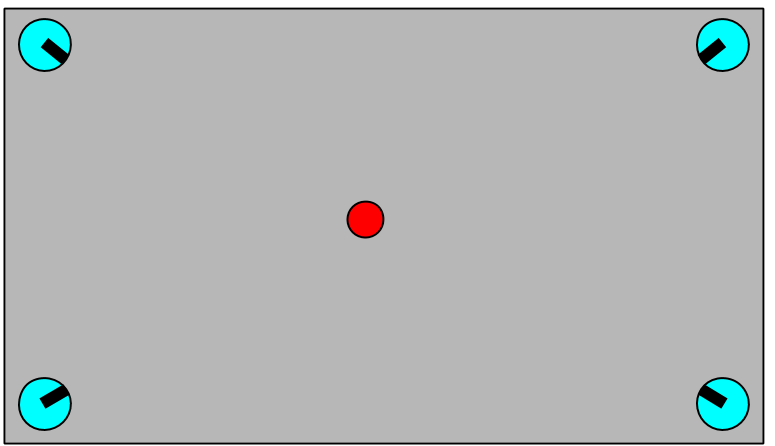
\includegraphics[width=0.8\linewidth]{figs/scenario0}
\end{center}
\caption[scenario 1]{Scenario 1, all the robots are placed in each corner with one obstacle}
\label{fig:scenario1}
\end{figure}

The first scenario is shown in figure \ref{fig:scenario1}, consists of four robots placed on each corner of the sandbox. The reason behind placing each of the robots in each corner of the sandbox is that each robot will be as far from each other as possible. This scenario should demonstrate that the entities are able to flock together, and then stay together as a flock. There is one obstacle placed nearby the middle of the sandbox, the obstacle is placed near the middle to ensure that the robots would encounter it at least once. This scenario would be able to see if the robots actually flocked together like they are supposed to do, and at the same time would be able to avoid the obstacle without bumping or crashing into it. The robots should also move together after they have flocked together.

\begin{figure}[h]
\begin{center}
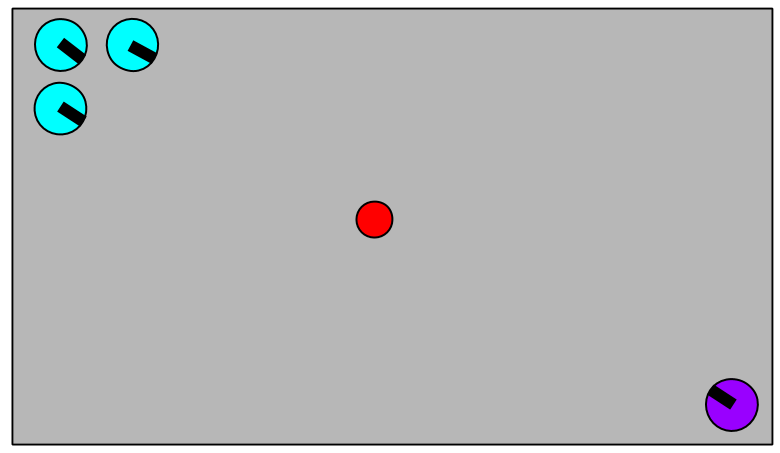
\includegraphics[width=0.8\linewidth]{figs/scenario1}
\end{center}
\caption[scenario 2]{Scenario 2, three robots in one corner, and the last one on the opposite corner}
\label{fig:scenario2}
\end{figure}

The second scenario puts three of entities in one corner, and the last entity is placed on the opposing corner as seen in figure \ref{fig:scenario2}. However the last entity that is placed on the lower right corner by itself will not move, in the case of the physical robot, it will not be turned on. The reason that this entity is a sitting duck placed on the opposite corner of all the other entities is that this robot will act as a goal for the other entities. The obstacle is placed between the lonely robot and the three robots that are clumped up together. The idea behind this setup is that the three robots that start together would try to move to the one that are stationary because they need to flock together. The robot that start by itself does not move because it is not turned on.
The obstacle in the middle will hinder the robots from moving in a straight line to their goal, which forces them to choose a way around it. The robots move around the obstacle when they approach it. As explained in section \ref{sec:robotArch}, the robots will turn either right or left randomly when moving directly towards an obstacle. The robots will probably move around the obstacle on each side of the obstacle, and flock together again on the other side when they have move past the obstacle.

The third scenario is a scenario where the robots are placed randomly around in the sandbox. The two first scenarios were designed for a specific purpose. The purpose of the third scenario is to demonstrate that the Boids behaviors are still intact, even when the robots are placed randomly in the sandbox. The position of the robots, where it should be placed and which way it is pointing was generated randomly by a random number generator. The starting point for this scenario is illustrated in figure \ref{fig:scenario3}. 

This scenario looks a little bit like the first scenario, the robots are laid out in the shape of a square. They are closer to each other than the robots in the first scenario. One of the robots are separated from the other by starting behind the obstacle, the robot can not move directly to the other three robots without first moving around the obstacle.
\begin{figure}[h!]
\begin{center}
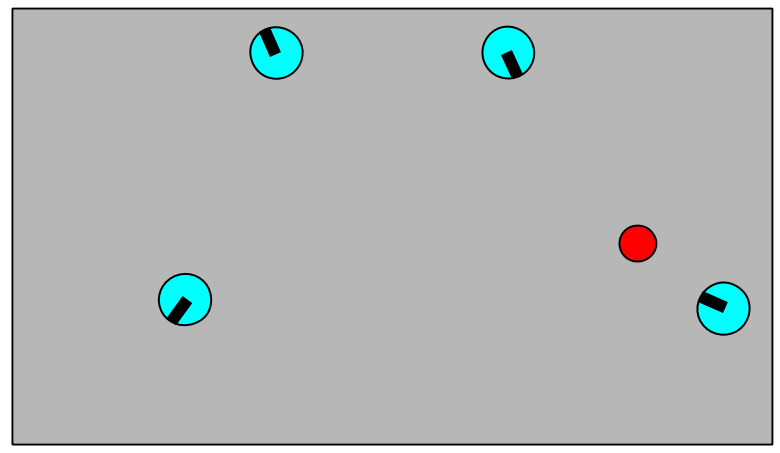
\includegraphics[width=0.8\linewidth]{figs/scenario2}
\end{center}
\caption[scenario 3]{Scenario 3, robots and obstacle randomly placed in the sandbox}
\label{fig:scenario3}
\end{figure}

All the scenarios explained in this thesis uses the same sandbox, which is a sandbox with the size of 151.6 cm wide and 123.9 cm long. The only difference between the scenarios are the placement and rotation of the robots and the placement of the obstacle. Each scenario were run ten times to generate the data seen in section \ref{sec:results}.
In between each run, the robots had to be placed manually back into their starting position before a new run could take place. To keep the data as consistent as possible, everything else would stay as exactly the same.
For the experiments on the simulator, only five runs will be used. Boids have the same starting position and the same direction each time, each run is therefore not very different from the other ones. 

The camera used in this experiment is a web camera. To be able to get a clear stable video feed images from the web camera, the settings for the camera had to be manually set up.
The most important setting is to disable auto focus. Auto focus makes the images blurry, and the camera tracking software will not be able to detect red and green colors which defines the robots. 50 Hz power line frequency was used instead of 60 Hz to eliminate flickering on the camera feed. The other settings are not that important, as long as the web camera is able to provide a decent looking image that the camera tracker software is able to recognize. 

%The experimental setup should include all data - parameters etc, that would allow a person to repeat your experiments. 


\section{Results}
\label{sec:results}

The Boids algorithm are supposed to keep the robots flocked together and preferably they should face the same direction as well. The watcher knows where each robot is, and it knows which direction each robot is facing. The watcher measures the distance between each robot and the angle difference between the robots every five frame or twelve times each second, it then calculates the mean and standard deviation of the distances and angles and saves it to a file. The mean and standard deviation of the velocity is recorded as well, in the simulator the velocity is measured directly by getting the velocity vector on each object, for the physical robot, the change in position is measured instead.

To keep the data as consistent between each run the watcher stops all the robots and saves the data file exactly three minutes or 180,000 milliseconds after the robots have started to move.
The distance measured are in pixels. The measurement of the sandbox is 151.6 cm wide and 123.9 cm long. The watcher software creates a window that has a resolution 800x652 pixels, which means that 1 cm is approximately 5.3 pixels on the screen. The measured angles are shown in radians.

In the upcoming figures, the results from the various runs will be shown. On the x-axis the time will be shown, and the y-axis displays various types of data is presented depending on the figure. The time shown on the x-axis displays the iteration, and not seconds. One iteration is five frames, the software runs with a 60 frames per second. Which means that twelve iterations on the x-axis corresponds to one second. The velocity is measured every iteration, the velocity graph is mostly used as an indication to whether the robots are moving or not. The velocity graphs can be used as an indication whether the robots are moving fast or slower, but it can not be used to reliably tell the velocity of the robots. The velocity graph for the simulated Boids are more precise.
The number shown on the y-axis shows the average length of the velocity vector for each Boid.

The upcoming figures will show graphs of various types, two similar ones will be displayed for each scenario. One is the results from ten runs on the physical experiment with the robots, and the other one is the results from the experiments ran in simulation. In section \ref{sec:discussion} a discussion of the results will be presented, it will contain an explanation as to why some of the graphs might be different.

\subsection{Results from scenario 1}
\label{sec:res1}
\begin{figure}[h]
\begin{center}
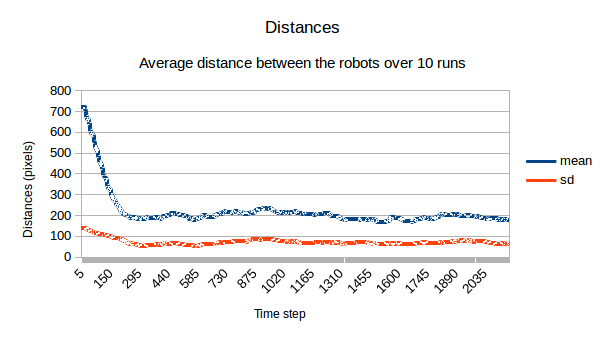
\includegraphics[width=0.8\linewidth]{figs/runs/1pdist}
\end{center}
\caption[1. Distances, robots]{Results from 10 runs averaged on scenario 1, robots}
\label{fig:res1pdist}
\end{figure}
\begin{figure}[h]
\begin{center}
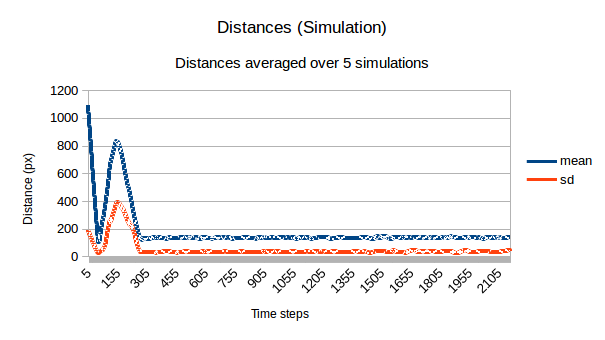
\includegraphics[width=0.8\linewidth]{figs/runs/1sdist}
\end{center}
\caption[1. Distances, simulation]{Results from 5 runs averaged on scenario 1, simulator}
\label{fig:res1sdist}
\end{figure}
%See figure \ref{fig:scene1peakillustrated}. %TODO
%\begin{figure}[h]
%\begin{center}
%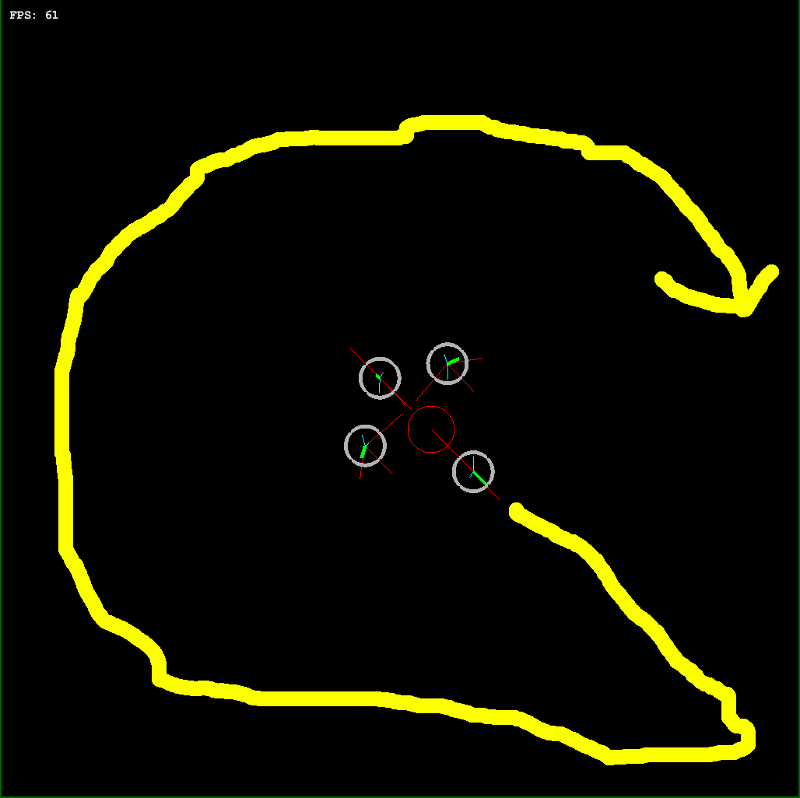
\includegraphics[width=0.8\linewidth]{figs/scene1_pushedaway2}
%\end{center}
%\caption[3. Velocity, robots]{Results from 10 runs averaged on scenario 3, simulator}
%\label{fig:scene1peakillustrated}
%\end{figure}
The first scenario was designed to check if the robots were able to flock together, the robots were placed on each of its corner, as far from each other as possible.
From the figure \ref{fig:res1pdist} we can see that the robots are flocking together quite fast, they start out on each corner of the sandbox then move towards the center of the sandbox, this is shown in the graph by the first drop from 700 px to around 200 px. This corresponds to roughly 132 cm to 37 cm. The time it takes for the graph to drop from 700 px to 200 px is around 300 iterations, which equals 25 seconds.
The simulated Boids behave differently in the same scenario, as seen from figure \ref{fig:res1sdist}, between time step 40 and 305, the graph shows a local maxima. Because all of the Boids are moving towards the middle due to the velocity they have at the start, the distance between them will decrease. But one of the Boids is moving directly toward the obstacle and facing it directly, when it comes too close, it will be "pushed" directly in the opposite direction. The Boid that is being "pushed" in the opposite direction by the obstacle is too far away from the other Boids for the cohesion behavior to be active, and therefore moves away from the rest of the flock. This is the reason there is a peak in the graph.

\begin{figure}[h]
\begin{center}
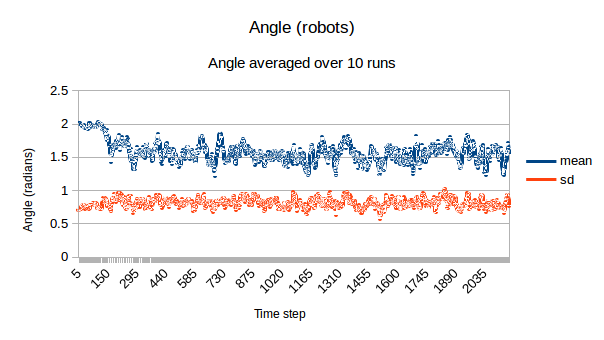
\includegraphics[width=0.8\linewidth]{figs/runs/1pangle}
\end{center}
\caption[1. Angle, robots]{Results from 10 runs averaged on scenario 1, robots}
\label{fig:res1pang}
\end{figure}
\begin{figure}[h]
\begin{center}
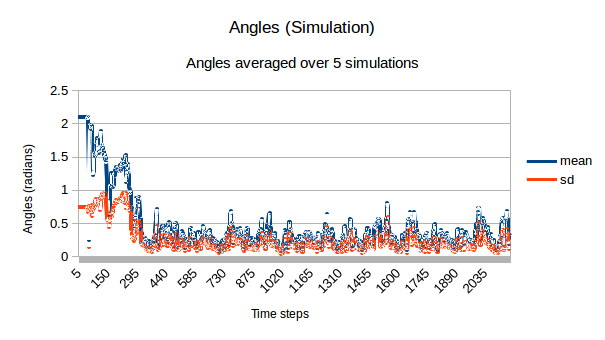
\includegraphics[width=0.8\linewidth]{figs/runs/1sangle}
\end{center}
\caption[1. Angle, Simulation]{Results from 5 runs averaged on scenario 1, simulator}
\label{fig:res1sang}
\end{figure}

In this scenario, the difference between the angles of the robots starts at 2 radians. This is when all of the robots are facing towards the center of the sandbox. After the robots have moved towards the center, they will start to turn around and the difference between the robots decreases. However, the robots are not able to face the same direction entirely, the lowest difference is still above 1.2 radians, which is approximately 68 degrees. 
The simulated Boids' angle also starts at approximately 2 radians, then slowly decreasing to 0.3 radians. %When the angle difference between the robots are 0.3 radians, they have flocked an 


\begin{figure}[h]
\begin{center}
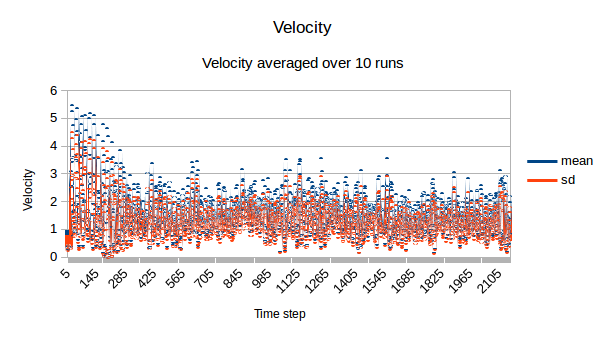
\includegraphics[width=0.8\linewidth]{figs/runs/1pvel}
\end{center}
\caption[1. Velocity, robots]{Results from 10 runs averaged on scenario 1, robots}
\label{fig:res1pvel}
\end{figure}
\begin{figure}[h]
\begin{center}
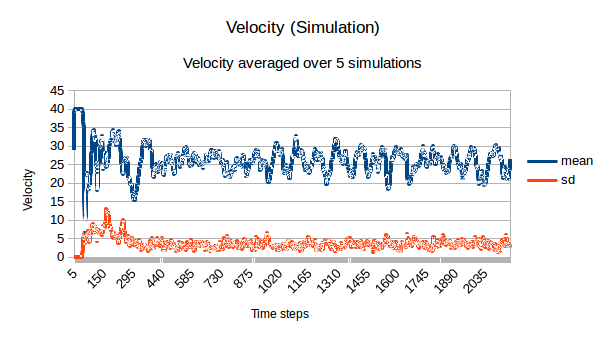
\includegraphics[width=0.8\linewidth]{figs/runs/1svel}
\end{center}
\caption[1. Velocity, simulation]{Results from 5 runs averaged on scenario 1, simulator}
\label{fig:res1svel}
\end{figure}
Both the robots and the Boids have high velocity at the start when they are moving towards the center. When the Boids reaches the center of the simulated space, they will need to adjust their velocity to change direction, and when all four Boids move together as a flock unit, they need to adjust their flight direction all the time. 
The velocity graph for the robot in this scenario has the same general outline as the simulated Boids; the graph shows a high velocity at the start, then drops down before stabilizing at a given range. The robots' velocity jiggles a lot, ranging 0.1 to 3.6, there might be various reasons for this result will be discussed more in depth in section \ref{sec:discussion}.
\clearpage
\subsection{Results from scenario 2}
\label{sec:res2}
\begin{figure}[h]
\begin{center}
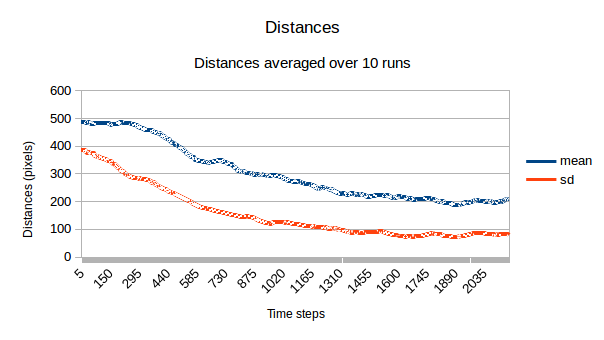
\includegraphics[width=0.8\linewidth]{figs/runs/2pdist}
\end{center}
\caption[2. Distances, robots]{Results from 10 runs averaged on scenario 2, robots}
\label{fig:res2pdist}
\end{figure}
\begin{figure}[h]
\begin{center}
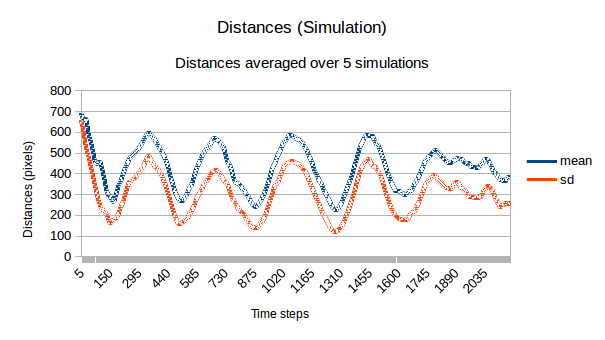
\includegraphics[width=0.8\linewidth]{figs/runs/2sdist}
\end{center}
\caption[2. Distances, simulation]{Results from 5 runs averaged on scenario 2, simulator}
\label{fig:res2sdist}
\end{figure}
Earlier demonstrations of Boids have shown us that when a flock of Boids are moving towards an obstacle, the Boids would split up to sub-groups, fly around the obstacle before merging together on the other side. This scenario is designed to check if this behavior is still intact.

In the second scenario, it takes a bit longer for the distance to drop to 200 px, around 1310 time steps, which is approximately 110 seconds.
Three of the robots are already in a flock while the fourth one is astray from the flock on the opposite side of the sandbox. The three robots that have already flocked together will try to stay together, they do not want to move all the way to the other side to flock with one single robot. If all of the robots were moving, the single robot would move towards the three robots and they all would flock together faster.

When running scenario 2 on the simulator, the Boids move towards the obstacle and around it. When they are near enough to the non-moving Boids, the cohesion behavior will activate and the Boids will try to flock, but all the other behaviors are trying to push the three moving Boids away from the non-moving Boid. After being pushed away, they will keep moving in the same direction and move all the way around the screen. This movement around the screen creates the oscillated graph seen in figure \ref{fig:res2sdist}.

\begin{figure}[h]
\begin{center}
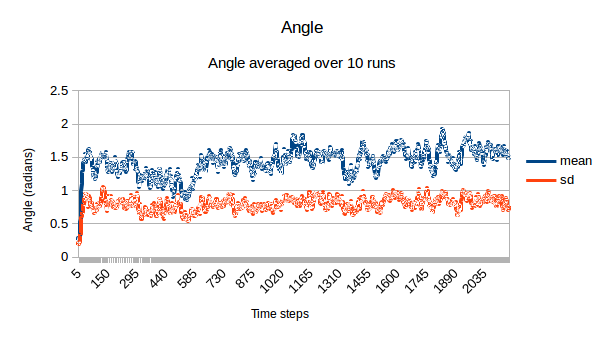
\includegraphics[width=0.8\linewidth]{figs/runs/2pangle}
\end{center}
\caption[2. Angle, robots]{Results from 10 runs averaged on scenario 2, robots}
\label{fig:res2pang}
\end{figure}
\begin{figure}[h]
\begin{center}
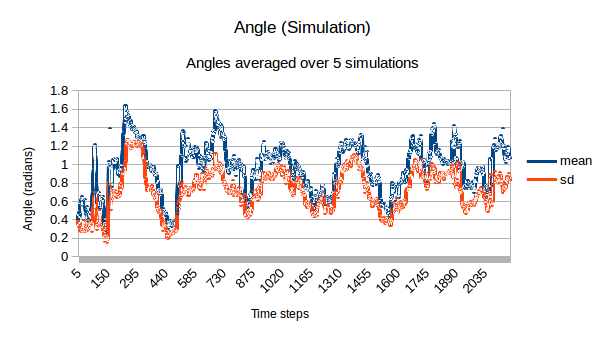
\includegraphics[width=0.8\linewidth]{figs/runs/2sangle}
\end{center}
\caption[2. Angles, robots]{Results from 5 runs averaged on scenario 2, simulator}
\label{fig:res2sang}
\end{figure}
In the second scenario, one of the entity is stationary, and thus its angle does not change, but its angle is still accounted for when the graphs were created. The angles shown in the graphs for the second scenario starts in the lower end, then increases.
Three of the entities starts by facing the same direction, while the last stationary one faces in the opposite direction. That is, all off them faces toward the center as seen in figure \ref{fig:scenario2}.
When starting the runs for the second scenario, the robots started to turn around immediately, thus increasing the difference-angle shown in the graph. One of the robot starts in the upper left corner, it is covered by the two other robot, having no way to move out of this corner without colliding into the other robots, its only option is to turn around on the spot.

The three moving Boids starts off by moving towards the center of the screen, they then move around the obstacle. After reaching the stationary Boid, they are pushed away, which forces them to turn away from the stationary Boid. The Boids angles follows a wave pattern, much like the distances.

\begin{figure}[h]
\begin{center}
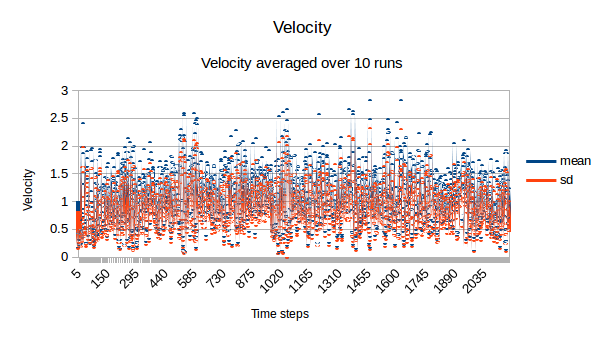
\includegraphics[width=0.8\linewidth]{figs/runs/2pvel}
\end{center}
\caption[2. Velocity, robots]{Results from 10 runs averaged on scenario 2, robots}
\label{fig:res2pvel}
\end{figure}
\begin{figure}[h]
\begin{center}
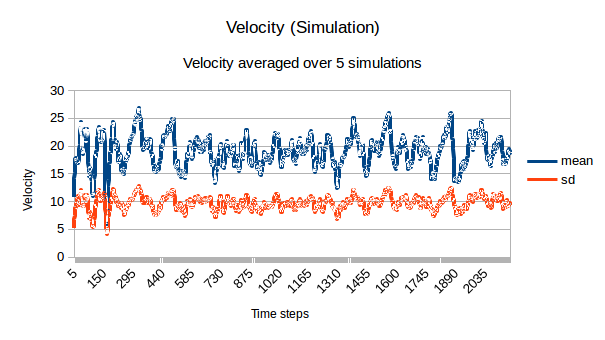
\includegraphics[width=0.8\linewidth]{figs/runs/2svel}
\end{center}
\caption[2. Velocity, robots]{Results from 5 runs averaged on scenario 2, simulator}
\label{fig:res2svel}
\end{figure}
Both of the velocity graphs in the second scenario are considerably lower than the ones found in the other two scenarios. This is expected because one of the four entity is stationary, i.e. non-moving. 
\clearpage
\subsection{Results from scenario 3}
\label{sec:res3}
\begin{figure}[h]
\begin{center}
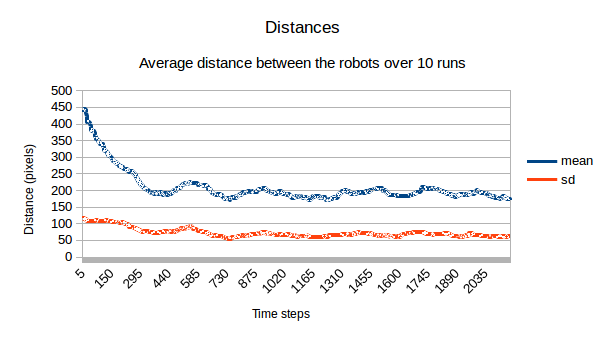
\includegraphics[width=0.8\linewidth]{figs/runs/3pdist}
\end{center}
\caption[3. Distances, robots]{Results from 10 runs averaged on scenario 3, robots}
\label{fig:res3pdist}
\end{figure}
\begin{figure}[h]
\begin{center}
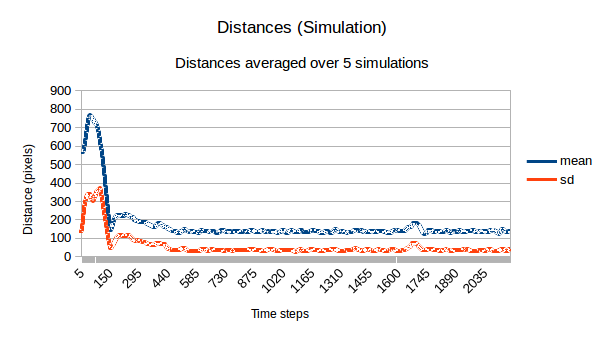
\includegraphics[width=0.8\linewidth]{figs/runs/3sdist}
\end{center}
\caption[3. Distances, simulation]{Results from 5 runs averaged on scenario 3, simulator}
\label{fig:res3sdist}
\end{figure}
The third scenario consists of entities that are placed randomly, the purpose behind this is to check that flocking and collision avoidance are still intact. Both the first and the second scenario were designed to check a specific behavior, this third scenario is not testing any specific behavior.

The results for the distances between the robots in the third scenario is similar to the one in the first. They move closer to each other, and then stay as a flock for the rest of the time. In the simulator, the Boids starts by moving further away from each other, before converging together.
The Boids that starts on the lower right are behind an obstacle, which pushes it away from the other ones. The lower left Boid has a start velocity away from the robots, and due to the short cohesion distance radius, it will move away from the other Boids. The other Boids are not in range for the cohesion behavior to activate.
However it does not take too long before the Boids are able to flock together, as seen from figure \ref{fig:res3sdist} the robots are starting to move towards each other after 40 time steps, and are fully flocked together at time step 150. 
The robots does not have the same behavior as the Boids in this scenario, and they have a much wider cohesion distance. Obstacles do not push the robots in the opposite direction either, when a robot tries to figure out which direction it is going to move in, it will ignore the wall and obstacles. If there is an obstacle in front of a robot, it will turn away from the obstacle. But the next time it calculates where it wants to go, it might calculate the direction it want to go is through the obstacle, thus the robot will turn toward the obstacle then realize that there is in fact an obstacle in front of it and it has to turn away. The robot might get stuck because of this turning behavior, but it will eventually force itself to move around the obstacle. In the mean time, the other robots will move towards the robot that has been stuck behind the obstacle.

The angle and velocity graph of the third scenario is relatively similar to the graphs in the first scenario.
\begin{figure}[h]
\begin{center}
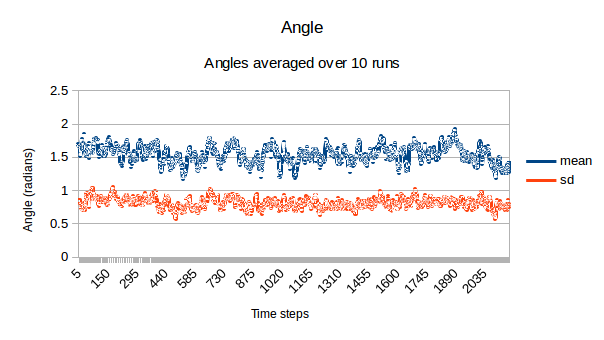
\includegraphics[width=0.8\linewidth]{figs/runs/3pangle}
\end{center}
\caption[3. Angle, robots]{Results from 10 runs averaged on scenario 3, robots}
\label{fig:res3pang}
\end{figure}
\begin{figure}[h]
\begin{center}
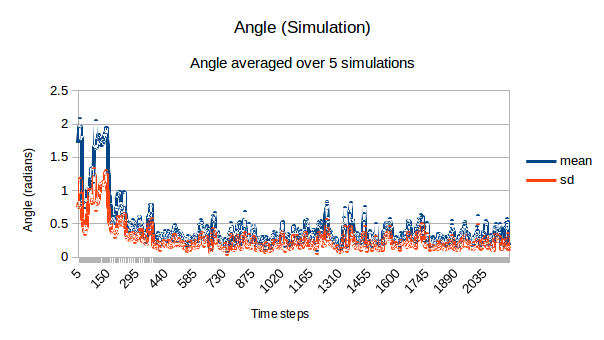
\includegraphics[width=0.8\linewidth]{figs/runs/3sangle}
\end{center}
\caption[3. Angle, robots]{Results from 5 runs averaged on scenario 3, simulator}
\label{fig:res3sang}
\end{figure}
\begin{figure}[h]
\begin{center}
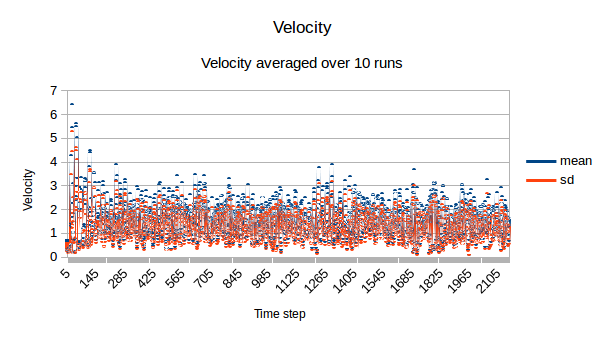
\includegraphics[width=0.8\linewidth]{figs/runs/3pvel}
\end{center}
\caption[3. Velocity, robots]{Results from 10 runs averaged on scenario 3, robots}
\label{fig:res3pvel}
\end{figure}
\begin{figure}[h]
\begin{center}
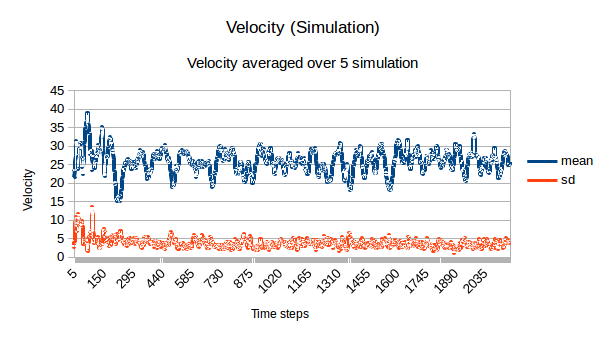
\includegraphics[width=0.8\linewidth]{figs/runs/3svel}
\end{center}
\caption[3. Velocity, robots]{Results from 5 runs averaged on scenario 3, simulator}
\label{fig:res3svel}
\end{figure}

\clearpage
\section{Discussion}
\label{sec:discussion}
This section will mainly focus on explaining the overall data from the results, why there is a difference between the physical experiment and the experiments done in a simulator.

The robots are able to flock faster in the first and third scenario than the robots in the second scenario. This might be because each of the robot start out by themselves and will therefore seek the other ones.
The equilibrium distance which the Boids are flocking at, seems to be around 120 px to 150 px. As mentioned earlier, the separation distance of the Boids is 120 px.
The separation distance for the robot is slightly increased compared to the Boids', the distance is 150 px instead of 120 px. The robots are not only influenced by the separation vector for collision avoidance, but they use their distance sensors as well. So it is expected that the equilibrium distance between the robot is not exactly at 150 px, according to the graphs, the robots' flocking distance stays around 200 px.
%The distances converges to 200 px in about 300-400 time steps for the robots in the first scenario and the third scenario. In the first and third scenario, the robots' distance converges to 200 px, and the simulator converges to 150 px. These numbers comes from the behaviors explained in section \ref{sec:experimentalSetup}. The separation distance is 120 px, so the Boids will try to stay around 120 px away from the other Boids. The same goes for the robot, but due to the distance sensors used for avoiding obstacles, they tend to stay further away from the other robots. 

%In the first and third scenario, each robot starts alone. Due to this, only the sensors used for obstacle avoidance, the "away from wall" and the cohesion behavior will be active. This makes each of the robot move towards the other ones, and the robots converge to a flock faster. 

%//angle
The angles measured seems to vary a lot, even if the alignment behavior tries to make all the robots face the same way. But the overall trend of the robots seems to be that the angles lingers around 1.5 radians on average for all three scenarios, which is pretty high.

The simulated Boids are able to face in the same direction as the other Boids, starting with an angle difference of 2 radians and slowly dropping down to 0.5 radians. This holds true on the graphs shown for the first and third scenario. The angles in second scenario are varying a lot, ranging from 0.4 radians to 1.6. This happens because one of the Boid is not moving, its angle is always 0. While the other three is moving around and their will range from $-\pi$ to $\pi$ depending on the direction they are moving.

If the allowed space to travel were bigger, and there were no obstacles. The Boids would be able to move without needing to turn, and the angle between them would stay consistently low. However the allowed space for the robots to travel is limited and there is an obstacle there as well.
Whenever the robots detects an obstacle or move towards the walls, the distance sensors will make the robot turn around so the robot will not crash. Sometimes the robots will think that the other robots around itself are obstacles as well, because it has no way to tell the difference between the robots from an actual obstacle. This is because the distance sensors can not distinguish anything, it only measures a distance and the robots will try to avoid anything that is too near it, thinking that the object it detects is an obstacle.

The velocity for the robot varies a lot, we can see from the graph that the velocity varies from 0 to 6.3. The watcher software logs the velocity data by finding the change in position between two time steps, that is it finds $\Delta P$ as shown in equation \ref{eq:calcrobvel} of each robot every iteration. When a robot is turning to change direction or to avoid an obstacle, it is not moving because it is just spinning in place. 

The method used to measure the velocity of the robot is very imprecise, when logging the velocity of a robot with constant max velocity, the results did not stay consistently at a given number. 

The result from this test is shown in figure \ref{fig:speed}, the robot is moving at max speed the whole time but there is no consistent line in the graph. The graph consists of "pillars", meaning that the graph goes from 12 to 0 and back up to 12 again. The big gaps in the graph is when the robot has encountered the wall and stops to turn away.

\begin{figure}[h]
\begin{center}
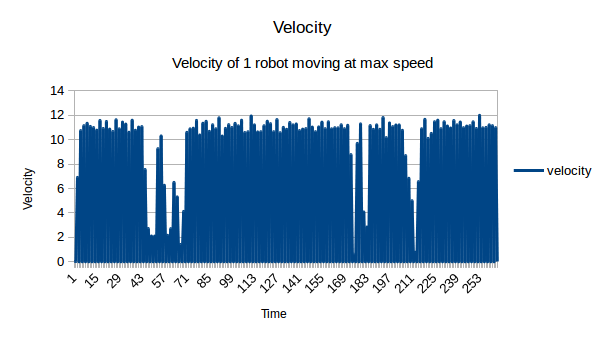
\includegraphics[width=0.8\linewidth]{figs/speed}
\end{center}
\caption[Velocity of robot]{One robot moving at max velocity, only turning when facing a wall}
\label{fig:speed}
\end{figure}

The Boids in the simulator never stops, that is why the velocity never drops down to 0, they keep moving in different direction all the time. Being able to move freely in all 360\textdegree\ almost instantly. They do not need to stop to change direction.
The physical ChIRP robot needs to turn around before moving in a new direction. As long as the new direction is off by an angle larger than 1\textdegree\ from the angle the robot is currently facing, then it will stop and turn. All turning takes approximately one second, before the robot is moving again. If the robot will turn a lot, it will only have one second to do so, before it has to move. If it only needs to turn 2\textdegree, it will turn first and wait until it has been one second before moving on.
The one second delay is introduced to keep the timing somewhat synchronous between the robots, one second delay is long enough for the robot to be able to almost turn all the way around (180\textdegree). 


The graphs only shows the average distance between the robots, the velocity of the robots and the difference between their angle. The graphs do not show where the robots are moving or whether they have crashed into anything.
Sometimes the robots do bump into the obstacles, or the other robots. The reason is that the robots measures the distances before moving, and not continuously while moving. So if a robot measures the distance in front of it and there is no obstacle in front of it, it will start to move forward. When the robot moves forward it might hit an obstacle or robot if the object is too close to it when it measures the distance. Sometimes robots moves onto the path of another robot while the other robot is moving, the other robot will probably bump into the one blocking its path. The robots do not crash into each other, that is they do not push each other around when they are trying to occupy the same space as the other robots. When the robots bump into each other, they nudge each other and might scrape against the surface of each other. However none of the paper taped on the robot has been torn apart when the robots were scraping against each other while running the experiment.

The robots only moves forward, and they only turn when they need to change direction or if there is an object in front of it that it needs to avoid. Sometimes the robots suddenly stops and rotates on the spot as if there is some sort of object in front of it, even if there is none.
Whenever the robot turns, the watcher will not see any change in position, which is the method it uses to log the velocity of the robots. The watcher will therefore log that the velocity of the robot is 0 when the robots turn around on the same spot. 
The distance measured by the robot's sensors might be imprecise, due to disturbances around in the room that makes the measured distances imprecise. The disturbances can come from the infrared light the other robots sends out when they are measuring distances themselves, which might bounce around in the sandbox and disturb the other robots. 

For the camera to see the two colored post it notes on the robots, the room needs to be well lit. Extra lights were placed around the sandbox to lit it up. The room where the experiment took place had two large windows, by daytime the sun would shine into the room. The sunlight contains infrared light, if the sun shines into the room and hits the area where the robots roam, the robot will sense the infrared lights from the sunshine and think that there is an object in front of it. The blinds in the room were closed, but some of the sun would always shine into the room.
